\documentclass[11pt,a4paper,twocolumn]{article}
\usepackage[a4paper,top=2.5cm,bottom=2.5cm,left=2.5cm,right=2.5cm,columnsep=0.6cm]{geometry}
\usepackage{times}
\usepackage[T1]{fontenc}
\usepackage[utf8]{inputenc}
\usepackage{microtype}
\usepackage[scaled=.88]{inconsolata}
\usepackage{array}
\usepackage{booktabs}
\usepackage{enumitem}
\usepackage{xcolor}
\usepackage{graphicx}
\usepackage{amsmath}
\usepackage[font=small,labelfont=bf,labelsep=period]{caption}
\usepackage[round]{natbib}
\usepackage{titlesec}
\usepackage{tikz}
\usetikzlibrary{arrows.meta,positioning,shapes.geometric,fit,backgrounds,calc}
\usepackage[colorlinks=true,linkcolor=blue!40!black,urlcolor=blue!40!black,citecolor=blue!40!black]{hyperref}

\renewcommand{\dbltopfraction}{0.9}
\renewcommand{\dblfloatpagefraction}{0.6}
\renewcommand{\topfraction}{0.9}
\renewcommand{\textfraction}{0.1}
\setlength{\dbltextfloatsep}{8pt plus 2pt minus 2pt}
\setlength{\parindent}{1em}
\setlength{\parskip}{0pt}
\setlength{\emergencystretch}{3em}
\setlist{nosep,leftmargin=1.3em}
\titleformat{\section}{\large\bfseries}{\thesection}{0.6em}{}
\titleformat{\subsection}{\normalsize\bfseries}{\thesubsection}{0.6em}{}
\titlespacing*{\section}{0pt}{1.1em}{0.4em}
\titlespacing*{\subsection}{0pt}{0.9em}{0.3em}
\titleformat{\paragraph}[runin]{\normalsize\bfseries}{}{0pt}{}[\ \ ]
\titlespacing*{\paragraph}{0pt}{0.45em plus 0.1em minus 0.1em}{0pt}
\renewcommand{\arraystretch}{1.08}

\tikzset{
  box/.style={draw, rounded corners=1pt, align=center, font=\tiny, text width=1.35cm, minimum height=0.62cm, inner sep=1.5pt, fill=blue!6},
  dbox/.style={draw, dashed, rounded corners=1pt, align=center, font=\tiny, text width=1.35cm, minimum height=0.62cm, inner sep=1.5pt, fill=gray!8},
  pbox/.style={draw, dashed, thick, rounded corners=1pt, align=center, font=\tiny, text width=1.35cm, minimum height=0.62cm, inner sep=1.5pt, fill=orange!14},
  lbl/.style={font=\tiny, align=center, text width=2.6cm},
  note/.style={font=\tiny\itshape, align=center},
  arr/.style={-{Latex[length=1.6mm]}, thick},
  darr/.style={-{Latex[length=1.6mm]}, dashed},
  dotarr/.style={-{Latex[length=1.3mm]}, dotted, thin},
}

\newcommand{\M}{\textsc{M}}
\newcommand{\Q}{\textsc{Q}}

\begin{document}

\twocolumn[{%
\begin{center}
{\Large\bfseries Beyond Streaming: Conversational Floor Control in Speech LLMs\\[0.2em]
and a Reproducible Telugu Speech-Pipeline Evaluation}\\[0.9em]
{\large Banuru Mohammed Fawaz}\\[0.15em]
{\normalsize Technical assignment, Speech AI Research Internship, Vaani Research Lab}\\[0.15em]
{\small Code: \url{https://github.com/f4w4z/vaani-technical-assignment}}\\[1.0em]
\begin{minipage}{0.88\textwidth}
\centering{\large\bfseries Abstract}\\[0.3em]
\small\raggedright
Speech language models are moving from turn-based cascades to streaming, full-duplex systems, yet ``real-time'' is usually reported as response-onset latency. We make two contributions. \emph{First}, we compare two recent speech LLMs, Moshi (full-duplex, speech-to-speech) and Qwen2.5-Omni (streaming, omni-modal, speech output), along seven architectural axes, record what their reports leave unspecified, and argue that streaming generation alone does not solve conversational \emph{floor control}: deciding to continue, hold, or yield while still listening. We split ``end-of-speech'' into four distinct decisions and specify, as a falsifiable experiment that we have \emph{not} run, a small controller on frozen Moshi that uses the model's own generation state to choose among them. \emph{Second}, we build and evaluate a reproducible Telugu speech-to-text-response cascade (Telugu-finetuned Whisper-small $\rightarrow$ Qwen2.5-1.5B-Instruct) with from-scratch metrics on 129 synthesized utterances in clean and 0\,dB-SNR conditions. Noise raises WER from 0.293 to 0.338 (paired 95\% CI of the increase: $+0.014$ to $+0.077$); a spectral-subtraction front end does not help ($\Delta$WER $+0.001$, CI $-0.014$ to $+0.017$). The dominant failure is the small LLM: it states the correct fact in 0 of 129 answers from speech and 3 of 129 from perfect transcripts, and never abstains. Code and configurations are released.
\end{minipage}
\vspace{1.2em}
\end{center}
}]

\section{Introduction}

A speech assistant feels conversational only if it answers quickly \emph{and} behaves sensibly about who holds the floor. Cascaded systems (ASR, text LLM, TTS) wait for an endpoint, so they cannot represent overlap or interruption. End-to-end streaming models such as Moshi \citep{moshi} and Qwen2.5-Omni \citep{qwenomni} remove that turn boundary and report low latency, but a latency number measures how soon speech \emph{starts}, not whether the system keeps talking through a listener's ``mm-hm'' or stops when it is genuinely interrupted.

This report has two parts that share a theme but make different kinds of claims, and we keep them apart.

\textbf{Part I (analysis and proposal; no experiments).} We analyze Moshi and Qwen2.5-Omni along the seven axes of the assignment brief, answer the research question of what architectural limitations prevent low-latency, natural, real-time conversation, and propose an improvement. Every statement about the models carries a section and page citation to the source report; everything beyond that is labeled interpretation or proposal.

\textbf{Part II (implementation and measurement).} We build and measure a \emph{cascaded} Telugu pipeline with our own evaluation code. This part does not test Part I's hypothesis: a cascade processes whole utterances and has no floor-control decision to evaluate. It supplies a measured baseline for what a modest, reproducible Indic system does today.

\paragraph{Contributions.}
(1) A comparative architectural analysis with an explicit list of unreported quantities that block matched comparison (\S\ref{sec:analysis}).
(2) A decomposition of end-of-speech into four decisions and a ranked account of three limitations (\S\ref{sec:limits}--\ref{sec:eos}).
(3) A fully specified, refutable proposal: a generation-state-aware yielding controller, with baselines, a constrained primary metric, and ablations (\S\ref{sec:proposal}).
(4) A reproducible Telugu cascade evaluation with from-scratch WER/CER/RTF, a defined correctness and hallucination rate, paired bootstrap intervals, and an honest negative result for a denoising extension (\S\ref{sec:system}--\ref{sec:results}).

\section{Related Work}

\paragraph{Duplex and streaming speech LMs.} dGSLM \citep{dgslm} models two-channel dialogue directly. Moshi \citep{moshi} adds a text-initialized backbone, a causal codec, and an ``inner monologue''. Mini-Omni \citep{miniomni} generates speech while reasoning in streaming fashion, and Qwen2.5-Omni \citep{qwenomni} pairs a Thinker with a Talker for text and speech output.

\paragraph{Turn-taking prediction.} TurnGPT \citep{turngpt} predicts turn shifts from text, and Voice Activity Projection \citep{vap} predicts future voice activity from audio. Turn prediction therefore predates our proposal; the question we pose is narrower (\S\ref{sec:proposal}). We have not exhaustively searched for prior controllers that read a speech generator's hidden state, so we make no priority claim.

\paragraph{Indic ASR and denoising.} Whisper \citep{whisper} and MMS \citep{mms} cover Telugu at differing quality, and community fine-tunes exist for individual Indic languages. Spectral subtraction \citep{boll} is a classical noise-suppression front end that we evaluate as a pre-ASR step.

%% ------------------------------------------------------------------ PART I
\section{Architectural Analysis of Two Speech LLMs}
\label{sec:analysis}

We chose Moshi and Qwen2.5-Omni because both are recent, both stream, and both produce speech (so the brief's speech-to-speech requirement is met twice over). Table~\ref{tab:axes} gives the seven-axis comparison and Figure~\ref{fig:architecture} the data flow. Citations are to the printed page numbers of the attached reports (\M{} = Moshi, \Q{} = Qwen2.5-Omni).

\begin{table*}[t]
\centering\footnotesize
\renewcommand{\arraystretch}{1.18}
\begin{tabular}{@{}>{\raggedright\arraybackslash}p{2.3cm}p{6.7cm}p{6.7cm}@{}}
\toprule
\textbf{Axis} & \textbf{Moshi} \citep{moshi} & \textbf{Qwen2.5-Omni} \citep{qwenomni} \\
\midrule
1. Encoder and representation learning &
Mimi: causal SeaNet convolutional codec (strides 4,5,6,8,2) with 8-layer causal Transformers before and after quantization; 24\,kHz audio to 512-d at 12.5\,Hz; 8 codebooks of 2{,}048 entries, 1.1\,kbps (\M{} \S3.3.1, pp.10--11). &
128-channel mel input (25\,ms window, 10\,ms hop), about 40\,ms per representation; audio encoder initialized from Whisper-large-v3 with block-wise attention (\Q{} \S2.2, p.4; \S3, p.6). \\
2. Semantic vs.\ acoustic representations &
Split quantizer: one semantic VQ distilled from WavLM (cosine loss, non-causal teacher used in training only) plus a 7-level acoustic RVQ, summed for reconstruction (\M{} \S3.3.2, p.12). &
Input: encoder representations. Output: discrete codes from \texttt{qwen-tts-tokenizer}; Talker is conditioned on Thinker hidden states (semantic) plus sampled text-token embeddings (phonetic) (\Q{} \S2.3, p.5). \\
3. Speech-to-LLM alignment &
No adapter: parallel token streams (both speakers' audio plus Moshi's own text) enter a Helium-initialized Temporal Transformer as summed learned embeddings; ``inner monologue'' aligns self-text via Whisper timestamps and PAD/EPAD tokens (\M{} \S3.4.1, \S3.4.4, pp.13--17). &
Adapters align the audio encoder to the Thinker LLM; they are trained first while the LLM is frozen. Talker consumes Thinker hidden states and text embeddings as a dual-track decoder (\Q{} \S2.1, p.3; \S3, p.6). \\
4. Streaming vs.\ non-streaming &
Causal 80\,ms frames; user and system streams modeled jointly so listening and speaking overlap; reported latency 160\,ms theoretical and 200\,ms practical (\M{} abstract, p.1; \S3.3.1, p.11). &
Block-wise input attention over 2\,s blocks; waveform decoding by a DiT over 4 blocks (2 lookback, 1 lookahead) and chunked BigVGAN; no numerical end-to-end latency reported (\Q{} \S2.4, p.5). \\
5. Autoregressive vs.\ non-autoregressive &
Hierarchical autoregression: Temporal Transformer over time, Depth Transformer over codebooks within a step; Mimi decodes the codes (\M{} \S3.4.1, pp.12--14). &
Thinker and Talker are autoregressive; mel generation is flow-matching (iterative, not token-by-token) followed by BigVGAN (\Q{} \S\S2.1--2.4, pp.3--5). \\
6. End-of-speech and stopping &
No utterance-end token: continuous streams represent speech or silence; PAD/EPAD structure text timing rather than command a stop (\M{} \S3.4.4, pp.16--17). &
Text EOS and ChatML message boundaries; interruption handling is not specified (\Q{} Fig.~2, p.3; \S4.1, p.6). \\
7. Training objectives and data &
Helium text pretraining (2.1T tokens), audio pretraining (7M hours, mostly English), multi-stream post-training, Fisher fine-tuning (2{,}000 h), synthetic instruction tuning ($>$20{,}000 h); cross-entropy with semantic weight 100, acoustic 1 (\M{} \S4, pp.17--21). &
Frozen-LLM alignment, then all-parameter training (800B image/video, 300B audio, 100B video-audio tokens), context 8k to 32k; Talker: continuation, DPO ranked by WER and punctuation-pause error, speaker tuning (\Q{} \S3, \S4.3, pp.6--7). \\
\bottomrule
\end{tabular}
\caption{Seven-axis comparison. Every cell is a statement from the cited report; consequences are discussed in the text.}
\label{tab:axes}
\end{table*}

\begin{figure*}[!tbp]
\centering
\begin{center}\footnotesize\textit{Reported model latency: 160\,ms theoretical; 200\,ms practical.}\end{center}
\resizebox{\textwidth}{!}{%
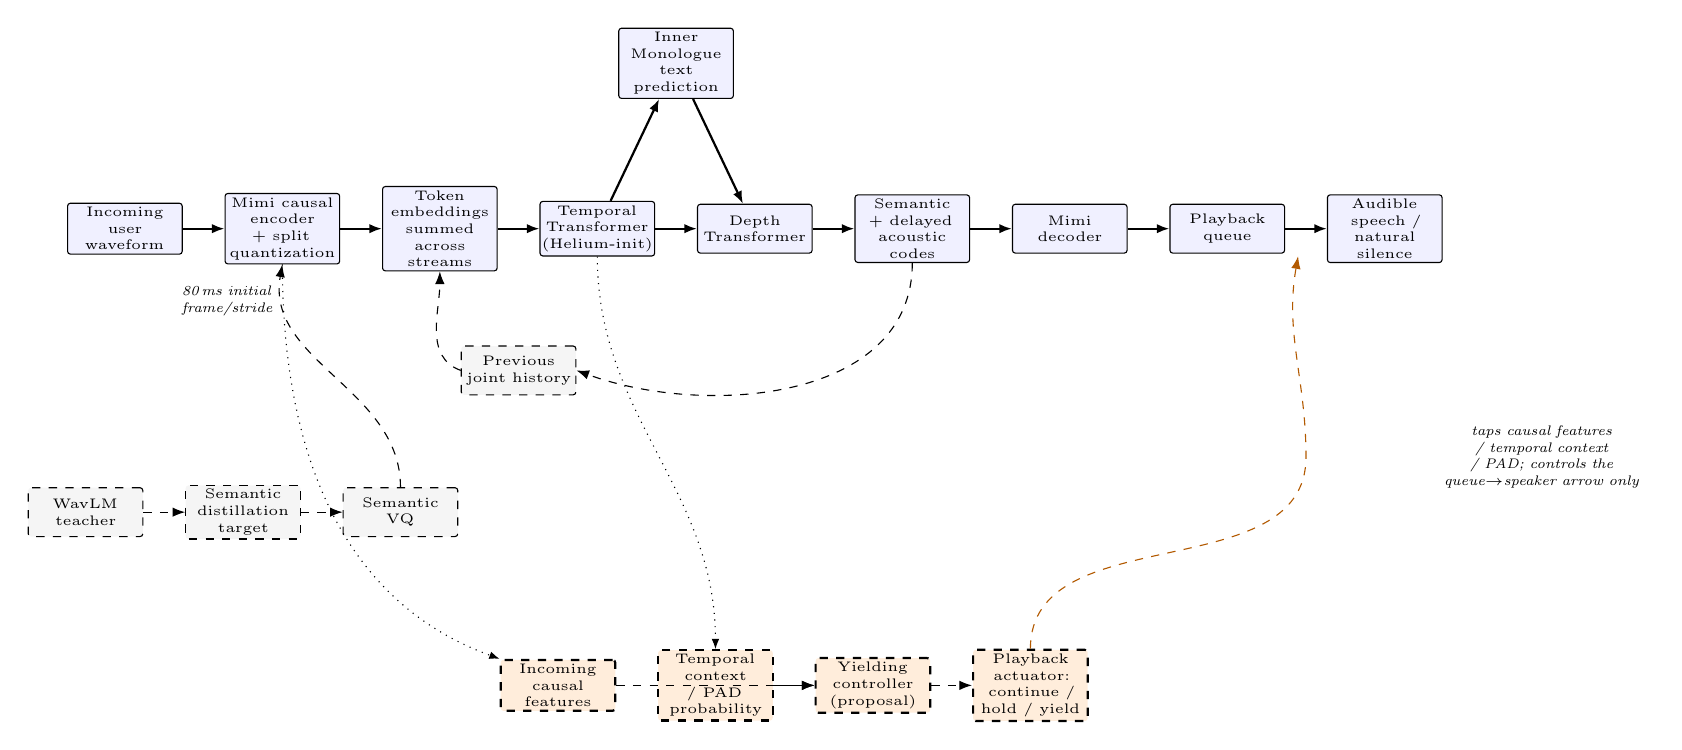
\begin{tikzpicture}
  % Panel A main chain (absolute grid: dx=2.0cm, main row y=0)
  \node[box] (a1) at (0,0) {Incoming user waveform};
  \node[box] (a2) at (2,0) {Mimi causal encoder + split quantization};
  \node[box] (a3) at (4,0) {Token embeddings summed across streams};
  \node[box] (a4) at (6,0) {Temporal Transformer (Helium-init)};
  \node[box] (a6) at (8,0) {Depth Transformer};
  \node[box] (a7) at (10,0) {Semantic + delayed acoustic codes};
  \node[box] (a8) at (12,0) {Mimi decoder};
  \node[box] (a9) at (14,0) {Playback queue};
  \node[box] (a10) at (16,0) {Audible speech / natural silence};
  \node[box] (a5) at (7,2.1) {Inner Monologue text prediction};
  \node[note, text width=2.0cm, anchor=north] at ([xshift=-0.7cm,yshift=-0.15cm]a2.south) {80\,ms initial frame/stride};

  \draw[arr] (a1) -- (a2);
  \draw[arr] (a2) -- (a3);
  \draw[arr] (a3) -- (a4);
  \draw[arr] (a4) -- (a5);
  \draw[arr] (a4) -- (a6);
  \draw[arr] (a5) -- (a6);
  \draw[arr] (a6) -- (a7);
  \draw[arr] (a7) -- (a8);
  \draw[arr] (a8) -- (a9);
  \draw[arr] (a9) -- (a10);

  % Feedback: previous joint history
  \node[dbox] (ah) at (5,-1.8) {Previous joint history};
  \draw[darr] (a7.south) to[out=-90,in=-20] (ah.east);
  \draw[darr] (ah.west) to[out=160,in=-90] (a3.south);

  % Training-only dashed branch
  \node[dbox] (wavlm) at (-0.5,-3.6) {WavLM teacher};
  \node[dbox] (distill) at (1.5,-3.6) {Semantic distillation target};
  \node[dbox] (semvq) at (3.5,-3.6) {Semantic VQ};
  \draw[darr] (wavlm) -- (distill);
  \draw[darr] (distill) -- (semvq);
  \draw[darr] (semvq.north) to[out=90,in=-100] (a2.south);

  % Proposal overlay (visually distinct, dashed orange)
  \node[pbox] (p1) at (5.5,-5.8) {Incoming causal features};
  \node[pbox] (p2) at (7.5,-5.8) {Temporal context / PAD probability};
  \node[pbox] (p3) at (9.5,-5.8) {Yielding controller (proposal)};
  \node[pbox] (p4) at (11.5,-5.8) {Playback actuator: continue / hold / yield};
  \draw[darr] (p1) -- (p3);
  \draw[darr] (p2) -- (p3);
  \draw[darr] (p3) -- (p4);
  \draw[dotarr] (a2.south) to[out=-90,in=160] (p1.north west);
  \draw[dotarr] (a4.south) to[out=-90,in=90] (p2.north);
  \draw[darr, orange!70!black] (p4.north) to[out=90,in=-90] (15,-2.9) to[out=90,in=-100] (14.9,-0.35);
  \node[note, text width=2.6cm] at (18,-2.9) {taps causal features / temporal context / PAD; controls the queue$\to$speaker arrow only};
\end{tikzpicture}}
\begin{center}\footnotesize Per-stage compute duration (encoder, Transformer, decoder, queue) is not individually reported; only the end-to-end figures above are stated. Dashed gray boxes are training-only; dashed orange boxes are the proposed controller, not an evaluated component.\end{center}

\vspace{0.4em}
\begin{center}\footnotesize\textit{Input: 2-second attention blocks (not an end-to-end latency measurement). DiT: 4-block context, 2 past + current + 1 future; future-block duration not reported.}\end{center}
\resizebox{\textwidth}{!}{%
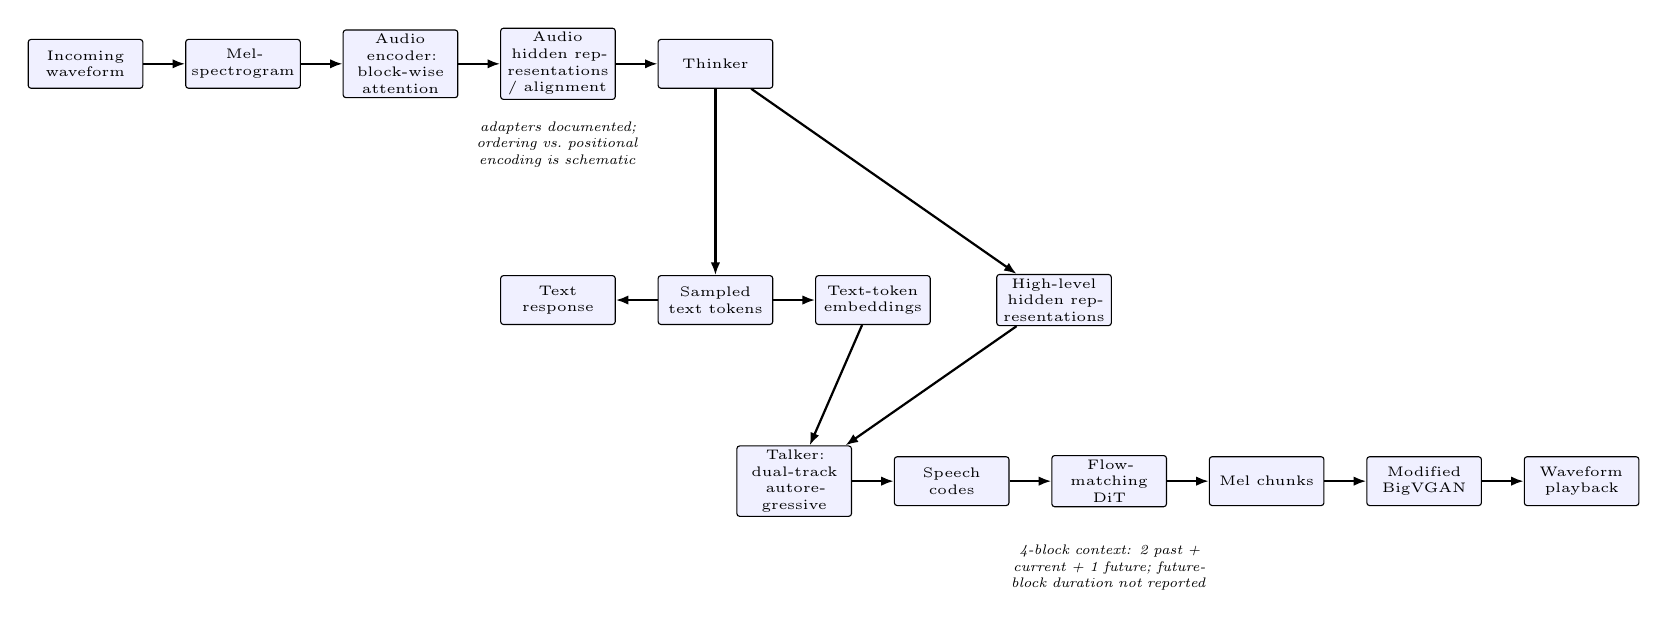
\begin{tikzpicture}
  \node[box] (b1) at (0,0) {Incoming waveform};
  \node[box] (b2) at (2,0) {Mel-spectrogram};
  \node[box] (b3) at (4,0) {Audio encoder: block-wise attention};
  \node[box] (b4) at (6,0) {Audio hidden representations / alignment};
  \node[box] (b5) at (8,0) {Thinker};
  \node[note, text width=2.6cm, anchor=north] at ([yshift=-0.15cm]b4.south) {adapters documented; ordering vs.\ positional encoding is schematic};

  \draw[arr] (b1) -- (b2);
  \draw[arr] (b2) -- (b3);
  \draw[arr] (b3) -- (b4);
  \draw[arr] (b4) -- (b5);

  \node[box] (b7) at (6,-3.0) {Text response};
  \node[box] (b6) at (8,-3.0) {Sampled text tokens};
  \node[box] (b9) at (10,-3.0) {Text-token embeddings};
  \node[box] (b8) at (12.3,-3.0) {High-level hidden representations};

  \draw[arr] (b5) -- (b6);
  \draw[arr] (b6) -- (b7);
  \draw[arr] (b6) -- (b9);
  \draw[arr] (b5) -- (b8);

  \node[box] (b10) at (9,-5.3) {Talker: dual-track autoregressive};
  \node[box] (b11) at (11,-5.3) {Speech codes};
  \node[box] (b12) at (13,-5.3) {Flow-matching DiT};
  \node[box] (b13) at (15,-5.3) {Mel chunks};
  \node[box] (b14) at (17,-5.3) {Modified BigVGAN};
  \node[box] (b15) at (19,-5.3) {Waveform playback};
  \node[note, text width=2.6cm] at (13,-6.4) {4-block context: 2 past + current + 1 future; future-block duration not reported};

  \draw[arr] (b9) -- (b10);
  \draw[arr] (b8) -- (b10);
  \draw[arr] (b10) -- (b11);
  \draw[arr] (b11) -- (b12);
  \draw[arr] (b12) -- (b13);
  \draw[arr] (b13) -- (b14);
  \draw[arr] (b14) -- (b15);
\end{tikzpicture}}
\begin{center}\footnotesize Per-stage compute duration and total onset delay are not reported in the source for either path.\end{center}
\caption{Architecture and timing dependencies. Top: Moshi (M §§3.3--3.4, pp.9--17; abstract, p.1). Bottom: Qwen2.5-Omni (Q §§2.1--2.4, pp.3--5; §3, p.6). Arrows show dependencies, not proportional execution durations. Solid = established pipeline; dashed gray = training-only path; dashed orange = the proposed yielding controller (a proposal, not a reported or evaluated component).}
\label{fig:architecture}
\end{figure*}

\paragraph{What the reports do not specify.} Neither report fully specifies input-endpoint, playback-completion/flush, or session-stop rules, and Qwen2.5-Omni additionally leaves interruption handling unspecified. Qwen2.5-Omni does not report output-codec rate, codebooks or bitrate; adapter dimensions or depth; output-block duration; numerical end-to-end latency; audio training hours or named corpora; or complete tokenizer objectives. Moshi's practical-latency figure comes without a complete measurement protocol, and Qwen's ``causal decoder'' wording sits beside a DiT with one lookahead block. These omissions prevent matched codec, latency, data-efficiency and stopping comparisons. They do not show a performance failure.

\section{Limitations Blocking Natural Real-Time Conversation}
\label{sec:limits}

Our answer to the research question is three ranked limitations. Each is interpretation built on the cited mechanisms, not a result reported by either paper.

\paragraph{L1. Continuous generation leaves conversational decisions implicit.} Moshi's joint streams remove the turn boundary and let the model listen while speaking (\M{} \S1, p.2; \S3.4.4, p.17). What remains open is \emph{when} that learned behavior correctly keeps or gives up the floor. Moshi evaluates gaps, overlaps and dialogue quality (\M{} \S5.6, p.31), but aggregate distributions cannot show whether one backchannel caused an inappropriate stop. Continuous modeling is a prerequisite for studying floor control, not evidence that it is handled well. Qwen2.5-Omni's streaming perception and generation likewise do not establish event-level behavior.

\paragraph{L2. Low transport delay does not establish timely social action.} Causal frames and hierarchical prediction (Moshi) or block-wise processing and bounded-context waveform decoding (Qwen) reduce the delay between input and output audio. Yet first-audio latency measures onset, not whether the system stops after a real interruption while talking through a backchannel. Suppressing output whenever speech appears yields fast stopping trivially, and refusing to stop yields few false yields trivially; neither is a better conversation. Any evaluation must therefore compare false yields only under common interruption-latency and missed-interruption limits, and the timing account must include input buffering, controller computation and playback queues. Because stage durations are unreported (above), a component-level timing diagram is more informative than comparing headline figures.

\paragraph{L3. Available cues and supervision may be insufficient.} Speech activity identifies that someone is making sound, not why. Distinguishing acknowledgment, hesitation and interruption needs context, and generation state (is the assistant finishing a phrase, waiting, or mid-explanation?) is a candidate cue whose usefulness must be tested. Supervision matters too: Moshi notes limits of simulated dialogue without overlap and Qwen acknowledges noisy speech supervision (\M{} \S4.4, pp.20--21; \Q{} \S4.3, p.7). A measured gain must therefore be attributed to a controlled intervention, not to differences between training corpora.

\section{End-of-Speech Is Four Decisions}
\label{sec:eos}

``End of speech'' conflates decisions that a conversational system must make separately (Table~\ref{tab:eos}). Moshi establishes continuous listening and generation including silence, while PAD/EPAD concern text timing, not a stand-alone stop command (\M{} \S3.4.4, pp.16--17). Qwen2.5-Omni establishes text and message boundaries and streaming waveform generation (\Q{} Fig.~2, p.3; \S\S2.3--2.4, p.5; \S4.1, p.6). Neither fully specifies the remaining boundaries.

\begin{table}[t]
\centering\footnotesize
\begin{tabular}{@{}p{1.75cm}p{2.7cm}p{2.7cm}@{}}
\toprule
\textbf{Decision} & \textbf{Meaning} & \textbf{Observable contrast} \\
\midrule
Input endpoint & User finished the current contribution & Hesitation pause vs.\ completed question \\
Conversational yield & Assistant gives the user the floor & Backchannel vs.\ genuine interruption \\
Output completion & Intended response finished playing & Intended end vs.\ playback and queue state \\
Session termination & Processing stops running & Explicit stop vs.\ ongoing listening \\
\bottomrule
\end{tabular}
\caption{Four decisions hidden inside ``end of speech''.}
\label{tab:eos}
\end{table}

Figure~\ref{fig:events} fixes the annotation targets. They are desired behaviors for a test, not assumed model behavior. A hesitation while the assistant has no active or pending output tests premature response onset and cannot count as a false yield; it is reported separately.

\begin{figure*}[!tbp]
\centering
\def\lanewidth{3.9cm}
\newcommand{\eventpanel}[6]{%
  \begin{tikzpicture}[node distance=0pt]
    \tiny
    \node[lbl, text width=1.9cm, anchor=east] (l1) at (0,0) {User audio};
    \node[lbl, text width=1.9cm, anchor=east] (l2) at (0,-0.5) {Assistant audio};
    \node[lbl, text width=1.9cm, anchor=east] (l3) at (0,-1.0) {Floor ownership};
    \node[lbl, text width=1.9cm, anchor=east] (l4) at (0,-1.5) {Controller action};
    \draw[draw=gray] (0.1,0.18) rectangle (0.1+\lanewidth,-0.18) ; #1
    \draw[draw=gray] (0.1,-0.32) rectangle (0.1+\lanewidth,-0.68) ; #2
    \draw[draw=gray] (0.1,-0.82) rectangle (0.1+\lanewidth,-1.18) ; #3
    \draw[draw=gray] (0.1,-1.32) rectangle (0.1+\lanewidth,-1.68) ; #4
    \node[note, below=2mm of l4, anchor=north west, xshift=-1.85cm, text width=6.2cm] {#5};
    \node[note, below=7mm of l4, anchor=north west, xshift=-1.85cm, text width=6.2cm] {#6};
  \end{tikzpicture}%
}
\begin{minipage}{0.48\textwidth}
\centering
\footnotesize\textbf{Hesitation pause}\\[2pt]
\eventpanel{
  \fill[blue!35] (0.1,0.18) rectangle (1.3,-0.18);
  \fill[blue!35] (2.3,0.18) rectangle (3.9,-0.18);
}{
  \fill[gray!15] (0.1,-0.32) rectangle (4.0,-0.68);
}{
  \node[font=\tiny] at (2.0,-1.0) {User (throughout)};
}{
  \node[font=\tiny] at (2.0,-1.5) {Hold -- do not start};
}{Label: \textit{``Endpoint control: do not start prematurely.''}}{False-yield analysis includes only episodes with active/pending assistant output and an independently annotated assistant floor.}
\end{minipage}
\hfill
\begin{minipage}{0.48\textwidth}
\centering
\footnotesize\textbf{Backchannel}\\[2pt]
\eventpanel{
  \fill[blue!35] (1.6,0.18) rectangle (2.2,-0.18);
}{
  \fill[orange!35] (0.1,0.18) rectangle (4.0,-0.18);
}{
  \node[font=\tiny] at (2.0,-1.0) {Assistant (throughout)};
}{
  \node[font=\tiny] at (2.0,-1.5) {Continue};
}{Label: \textit{``Continue; do not yield solely because speech is detected.''}}{}
\end{minipage}

\vspace{0.6em}
\begin{minipage}{0.48\textwidth}
\centering
\footnotesize\textbf{Genuine interruption}\\[2pt]
\eventpanel{
  \fill[blue!35] (1.9,0.18) rectangle (4.0,-0.18);
}{
  \fill[orange!35] (0.1,0.18) rectangle (2.2,-0.18);
}{
  \node[font=\tiny] at (1.0,-1.0) {Assistant};
  \node[font=\tiny] at (3.0,-1.0) {User};
}{
  \node[font=\tiny] at (2.0,-1.5) {Yield};
}{Marked interval: \textit{``Interruption-to-yield latency: measured in experiment.''}}{}
\end{minipage}
\hfill
\begin{minipage}{0.48\textwidth}
\centering
\footnotesize\textbf{Completed question}\\[2pt]
\eventpanel{
  \fill[blue!35] (0.1,0.18) rectangle (2.0,-0.18);
}{
  \fill[orange!35] (2.1,0.18) rectangle (4.0,-0.18);
}{
  \node[font=\tiny] at (1.0,-1.0) {User};
  \node[font=\tiny] at (3.0,-1.0) {Assistant};
}{
  \node[font=\tiny] at (2.0,-1.5) {Answer onset};
}{Label: \textit{``Answer onset; distinct from interruption yielding.''}}{}
\end{minipage}
\caption{Conversational events and desired actions. Four lanes per panel: user audio, assistant audible audio, desired floor ownership, desired controller action. Time is symbolic (no numerical durations). These are desired behaviors for the proposed test, not measured traces.}
\label{fig:events}
\end{figure*}

\section{Proposal: Generation-State-Aware Yielding}
\label{sec:proposal}

\paragraph{Hypothesis.} \emph{A frozen speech LLM's own generation state improves continue/hold/yield decisions beyond incoming audio and observable playback history, predicting fewer false yields on eligible backchannel and hesitation events than speech-activity rules and an audio-only learned controller, under matched interruption-to-yield latency and missed-interruption constraints.} It is refuted if the state-aware controller cannot improve that constrained comparison on held-out speakers and conversations, or if removing generation state preserves the benefit. This is a proposal: \textbf{no result is claimed.}

\paragraph{Controller.} Attach a small causal controller to \emph{frozen} Moshi. Inputs are current Mimi representations and causal speech-activity features, observable assistant playback activity, elapsed activity and silence durations, and queue occupancy. The generation-state additions are the Temporal Transformer context vector and the self-text PAD probability (\M{} \S3.4.1, pp.13--14; \S3.4.4, pp.16--17); whether an implementation exposes them must be verified. Only values available at decision time enter the controller. A learned projection and recurrent classifier output \textbf{continue} (release audio), \textbf{hold} (briefly suspend release, keep listening) or \textbf{yield} (suppress output, clear pending playback, keep listening, resume only on a later decision), all through one bounded playback actuator. Hold duration is capped on development data and inappropriate holding counts as disruption, not as a successful non-yield. The contribution under test is the use of generation state, not turn-taking prediction itself.

\paragraph{Training and data.} Only the projection and classifier are trained, with action cross-entropy. Labels give event type, floor ownership, onset, acceptable action intervals and interruption deadlines; annotators hear surrounding dialogue and mark ambiguity independently of controller output, and future context may inform labels but never inputs. Data are consented human--Moshi conversations and controlled reenactments recorded as separate user and played-assistant channels, replayed through frozen Moshi for causal feature traces, with Fisher's separate channels a possible auxiliary source for human cues (\M{} \S4.2, p.18). Splits are by speaker, conversation and scenario; thresholds and hold limits are chosen on development data only.

\paragraph{Baselines and primary metric.} We compare unmodified Moshi, a prespecified fixed-threshold speech-activity rule, a development-tuned rule, an audio-only learned controller, and the state-aware controller (Figure~\ref{fig:matrix}), all with the same actuator. The primary metric is the unweighted mean of false-yield rates over eligible backchannels and hesitations, where a hold exceeding the annotated tolerance counts as equivalent disruption. Operating points are compared only under common limits on interruption-to-yield latency (annotated onset to actual playback cessation) and missed-interruption rate, set from development-set baseline behavior \emph{before} testing. If no operating point meets both, the benefit is unsupported. Uncertainty is estimated by resampling conversations.

\paragraph{Ablation, robustness, controls.} The diagnostic ablation removes generation-state features but keeps acoustic features, playback history, queue state, capacity and training budget, so any remaining benefit is attributable to a learned audio policy or to knowing that the assistant is speaking. Robustness repeats held-out events under identical noise and echo perturbations and adds a Hindi/Telugu subset with fluent annotators, reporting zero-shot transfer separately from adaptation. Checkpoint, generation settings, hardware, recordings, actuator and annotation protocol are held fixed.

\paragraph{Threats.} Generation state may encode only timing or speaker identity (addressed by supplying playback history to both learned variants and by speaker-disjoint splits); gains may come from extra waiting (latency constraints and hold accounting); and scripted cues may not transfer (natural held-out conversations). Moshi can also generate speech internally that suppression keeps the user from hearing, so freezing the model does not repair its internal dialogue state; we track unheard output, resumption coherence and controller overhead as follow-up outcomes.

\begin{figure*}[!tbp]
\centering
\footnotesize
\begin{tabular}{c c c}
\tikz\node[draw, circle, fill=blue!15, inner sep=3pt, font=\tiny]{BC}; Backchannel &
\tikz\node[draw, circle, fill=orange!20, inner sep=3pt, font=\tiny]{HES}; Hesitation &
\tikz\node[draw, circle, fill=red!15, inner sep=3pt, font=\tiny]{INT}; Interruption \\
\end{tabular}

\vspace{0.4em}
\begin{tabular}{@{}l c c c l@{}}
\toprule
\textbf{Condition} & \textbf{Audio cues} & \textbf{Playback history} & \textbf{Moshi state} & \textbf{Threshold selection} \\
\midrule
Unmodified Moshi & Native & Native & Native & No added controller \\
Fixed speech-activity rule & Yes & Same actuator & No & Prespecified \\
Tuned speech-activity rule & Yes & Same actuator & No & Development set \\
Audio-only learned controller & Yes & Yes & No & Development set \\
State-aware learned controller & Yes & Yes & Yes & Development set \\
\bottomrule
\end{tabular}

\vspace{0.5em}
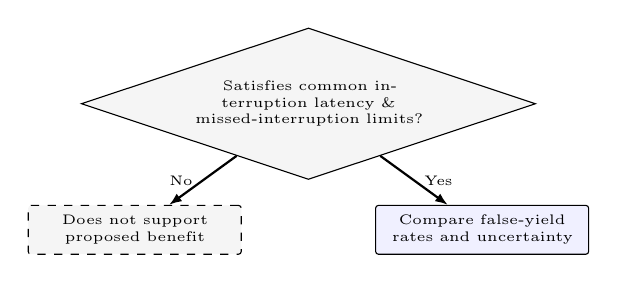
\begin{tikzpicture}[node distance=5mm]
  \node[draw, diamond, aspect=3, align=center, font=\tiny, text width=3.1cm, fill=gray!8] (gate) {Satisfies common interruption latency \& missed-interruption limits?};
  \node[dbox, below left=8mm and -6mm of gate, text width=2.6cm] (no) {Does not support proposed benefit};
  \node[box, below right=8mm and -6mm of gate, text width=2.6cm] (yes) {Compare false-yield rates and uncertainty};
  \draw[arr] (gate) -- node[left, font=\tiny] {No} (no);
  \draw[arr] (gate) -- node[right, font=\tiny] {Yes} (yes);
\end{tikzpicture}

\vspace{0.4em}
\begin{minipage}{0.47\textwidth}
\fbox{\parbox{0.92\linewidth}{\footnotesize\textbf{Held fixed:} checkpoint, generation settings, hardware, recordings, actuator, annotation protocol.}}
\end{minipage}
\hfill
\begin{minipage}{0.47\textwidth}
\fbox{\parbox{0.92\linewidth}{\footnotesize\textbf{Separate checks:} noise/echo robustness; Hindi/Telugu transfer; resumption coherence.}}
\end{minipage}
\caption{Experimental design matrix. No empirical curve is implied; all rows are proposed conditions, not measured results.}
\label{fig:matrix}
\end{figure*}

%% ----------------------------------------------------------------- PART II
\section{A Reproducible Telugu Speech Pipeline}
\label{sec:system}

\paragraph{System.} Speech $\rightarrow$ Whisper-family ASR $\rightarrow$ instruction LLM $\rightarrow$ Telugu text response, with both models resident on one GPU and reused across the run. Latency is wall-clock per sample with CUDA synchronization, including audio decoding and resampling but excluding model loading.

\paragraph{Model choice under a memory budget.} The evaluation GPU (RTX 4060 Laptop, 8\,GB) had about 6.5\,GB free, too little for the originally configured Whisper-large-v3 (about 3\,GB fp16) with Qwen2.5-7B-Instruct (about 15\,GB). We used \texttt{vasista22/whisper-telugu-small}, a Telugu-only community fine-tune of Whisper-small, and Qwen2.5-1.5B-Instruct \citep{qwen25}. The substitution of the fine-tune was forced: the general \texttt{openai/whisper-small}, even with Telugu forced, emitted Devanagari-looking text for Telugu audio and looped on short clips. Our first full run under it had corpus WER 2.56 and was discarded. The fine-tune's \texttt{generation\_config.json} predates \texttt{transformers}' \texttt{language}/\texttt{task} validation and raises \texttt{ValueError} if either is passed at all (reproduced on \texttt{transformers} 5.15.0 and 4.57.6), so our wrapper treats \texttt{language: null} as ``pass neither''.

\paragraph{Data.} No Telugu speech corpus was available locally, so we synthesized one: 129 template questions with reference answers, comprising 29 Indian state/UT capitals and 100 addition problems spoken as Telugu number words (1--10), rendered with \texttt{facebook/mms-tts-tel} \citep{mms}. Two corpora share this text: \textbf{clean}, and \textbf{noisy}, with additive white Gaussian noise at 0\,dB SNR (noise power equals signal power). An earlier 8\,dB corpus changed WER by under 0.002 and was replaced because it exposed no bottleneck. Both exceed the 100-example requirement and give two acoustic conditions. The corpora are \emph{not} byte-identical pairs: TTS duration prediction was unseeded and the noisy set was regenerated, so the clean/noisy gap includes rendering variance. The noisy-baseline vs.\ denoised comparison reuses identical audio and is exactly matched.

\paragraph{Evaluation infrastructure (from scratch).} WER and CER come from our own unit-cost Levenshtein implementation over NFC-normalized text; corpus rates divide total edits by total reference length, and CER counts Unicode code points without whitespace. Real-time factor (RTF) is pipeline seconds over audio seconds. Response quality is multiset word-overlap F1, computed both for the answer from the ASR transcript and for the answer from the human transcript, which isolates ASR's downstream effect. Greedy decoding keeps the paired comparison deterministic.

\paragraph{Correctness and hallucination rate.} Every reference answer states one checkable fact (a capital name or a sum word). An answer is \emph{correct} if it contains that fact (sums also accept the digit form, matched as a whole number), \emph{abstained} if not correct but containing an uncertainty marker (Telugu for ``don't know'', ``sorry'', ``not clear''), and \emph{hallucinated} otherwise: a wrong or off-topic answer asserted without hedging despite the prompt's ``ask for clarification, do not invent facts''. The test is lexical, so a correct answer in a different inflection is miscounted, making the rate an upper bound.

\paragraph{Uncertainty.} Differences between systems are reported with 95\% paired bootstrap intervals (10{,}000 resamples over the 129 questions, paired by question).

\section{Results}
\label{sec:results}

All runs completed 129 of 129 samples with no failures.

\begin{table}[t]
\centering\footnotesize
\begin{tabular}{@{}lrrr@{}}
\toprule
 & \textbf{Clean} & \textbf{Noisy} & \textbf{Noisy+DN} \\
\midrule
Corpus WER & 0.293 & 0.338 & 0.339 \\
Corpus CER & 0.075 & 0.096 & 0.099 \\
ASR time (s) & 1.74 & 2.05 & 2.03 \\
LLM time (s) & 12.71 & 15.42 & 15.28 \\
Total time (s) & 14.45 & 17.47 & 17.31 \\
Pipeline RTF & 4.15 & 4.99 & 4.95 \\
ASR-only RTF & 0.50 & 0.59 & 0.58 \\
F1 (ASR input) & 0.166 & 0.155 & 0.155 \\
F1 (human input) & 0.169 & 0.169 & 0.169 \\
\bottomrule
\end{tabular}
\caption{Baseline results (129 samples each). Noisy is 0\,dB SNR; DN is spectral-subtraction denoising. Times are means. The human-transcript F1 is the same reference arm in every column.}
\label{tab:main}
\end{table}

\subsection{Noise Degrades ASR; the LLM Dominates Latency}

Noise raises corpus WER from 0.293 to 0.338 and CER from 0.075 to 0.096 (Table~\ref{tab:main}). The paired bootstrap places the WER increase at $+0.045$ (95\% CI $+0.014$ to $+0.077$) and the CER increase at $+0.022$ ($+0.008$ to $+0.036$), so the effect is real even though the renderings differ. The ASR stage is comfortably real time (RTF 0.50), but the full pipeline is not (RTF 4.15 to 4.99) because the LLM stage accounts for about 88\% of pipeline time in both conditions. That share is a property of our setup (a 1.5B model on a laptop GPU, greedy decoding, up to 256 new tokens), not of cascades in general.

\subsection{Correctness and Hallucination}

\begin{table}[t]
\centering\footnotesize
\begin{tabular}{@{}llrrr@{}}
\toprule
\textbf{Condition} & \textbf{Input} & \textbf{Corr.} & \textbf{Abst.} & \textbf{Halluc.} \\
\midrule
Clean & ASR & 0 & 0 & 129 \\
Clean & human & 3 & 0 & 126 \\
Noisy & ASR & 0 & 0 & 129 \\
Noisy & human & 3 & 0 & 126 \\
Noisy+DN & ASR & 0 & 0 & 129 \\
Noisy+DN & human & 3 & 0 & 126 \\
\bottomrule
\end{tabular}
\caption{Answer correctness out of 129. The hallucination rate is 1.000 from ASR input and 0.977 from human transcripts in every condition.}
\label{tab:halluc}
\end{table}

The LLM, not the ASR, is the dominant failure. Even given the perfect transcript, only 3 of 129 answers state the right fact and mean F1 is 0.169; exact-match is 0 of 129 everywhere. The model \emph{never abstains} (0 of 774 answers across six arms), so every miss is a confident non-answer or wrong answer, typically fluent, repetitive Telugu that restates the question without naming the capital. ASR errors add little on top: the F1 gap between human and ASR input is 0.003 (clean) to 0.014 (noisy). The smallest Qwen2.5 checkpoint therefore fails at Telugu factual recall and instruction following in this setup, and a larger model, ruled out here by memory, would be the first remedy.

\subsection{Research Extension: Denoising as a Bottleneck Fix}

Given the measurable noise penalty, we implemented magnitude spectral subtraction \citep{boll} as a pre-ASR step: a per-frequency noise floor from a low time-percentile of STFT magnitude, subtracted with a floor to limit musical noise, then resynthesis with the original phase. Table~\ref{tab:dn} compares it with the baseline on identical audio.

\begin{table}[t]
\centering\footnotesize
\setlength{\tabcolsep}{3pt}
\begin{tabular}{@{}lrr@{}}
\toprule
\textbf{Comparison} & $\Delta$ & \textbf{95\% CI} \\
\midrule
Corpus WER & $+0.0014$ & $[-0.014, +0.017]$ \\
Corpus CER & $+0.0028$ & $[-0.004, +0.010]$ \\
\midrule
\multicolumn{3}{@{}l}{\textit{25-question ASR-only sweep (mean WER)}} \\
No denoising & 0.543 & \\
Mild ($\alpha{=}1.5$, floor 0.05) & 0.530 & \\
Aggressive ($\alpha{=}3.0$, floor 0.02) & 0.557 & \\
\bottomrule
\end{tabular}
\caption{Denoising ablation on identical noisy audio; $\Delta$ is denoised minus not denoised. Both intervals contain zero. The sweep covers the first 25 questions only (capitals), and ``mild'' is the shipped default.}
\label{tab:dn}
\end{table}

\paragraph{The fix did not help.} At default settings WER and CER moved by $+0.001$ and $+0.003$, with intervals comfortably containing zero, so we cannot distinguish the effect from sampling noise. A small subset sweep shows mild subtraction helping slightly and aggressive subtraction hurting, consistent with over-subtraction introducing musical-noise artifacts that a neural recognizer handles worse than the original stationary noise; with only 25 questions this is suggestive, not established. The filter does what it should at signal level (RMS 0.228 to 0.177; squared error to an independent clean rendering 0.094 to 0.073 on one sample), so the negative result concerns whether that cleanup survives through the recognizer, not whether the code works. Latency overhead was negligible (mean ASR time 2.05\,s vs.\ 2.03\,s).

\begin{figure*}[!tbp]
\centering
\includegraphics[width=0.48\textwidth]{../outputs/plots/clean/wer_vs_quality.png}\hfill
\includegraphics[width=0.48\textwidth]{../outputs/plots/clean/latency_breakdown.png}
\caption{Clean condition. Left: per-sample WER against response F1 for ASR-transcript and human-transcript inputs (many samples share a WER because questions are short). Right: mean latency; the LLM stage dominates. Noisy-condition plots are in Appendix~\ref{app:plots}.}
\label{fig:plots}
\end{figure*}

\section{Discussion}

The two parts meet at one observation: neither a faster first token nor a cleaner front end addresses what actually limits these systems. In Part I, headline latency says little about floor control; in Part II, where a cascade has no floor-control decision at all, the measured bottlenecks were the LLM's factual reliability and its generation time, with acoustic noise a smaller and (via our denoiser) not-yet-remedied third. We caution against reading Part II as support for Part I: they test different systems.

For the proposal, Part II offers a practical lesson about evaluation design. Our first plausible-looking configuration produced a WER of 2.56 and our first noise level produced no effect; both were visible only because the harness reports per-sample outputs and a clean-versus-ASR comparison. We would build the same safeguards (state-removal ablation, matched constraints, held-out speakers) into any run of the yielding experiment before trusting its primary metric.

\section*{Limitations}

\textbf{Part I is analysis and a proposal; it contains no experiment and claims no gain, dataset size, parameter count or runtime.} Statements about the models rest on the two attached reports and may not reflect later releases. Implementation access to Moshi's temporal context and PAD probability, Fisher licensing, and the effect of suppressing audio on Moshi's internal state remain to be verified, and novelty of the state-aware combination is unchecked.
\textbf{Part II} uses synthetic TTS speech, not real speakers, so it says nothing about accent, prosody or channel variation. The models are small because of a 6.5\,GB memory budget and would likely change both the WER and the factual accuracy substantially at larger scale. Clean and noisy corpora are not matched recordings. Response quality is a lexical proxy and the hallucination check is a substring heuristic, not a semantic judge. Results are from a single deterministic greedy run per condition, with intervals reflecting only question sampling. The ASR checkpoint's revision is unpinned because its configuration files and weights resolved to two different \texttt{main} commits within one session, and pinning either broke loading.

\section*{Ethical Considerations}

All evaluation audio is machine-synthesized from template text, so no personal data or human recordings were collected. The proposed human--Moshi data collection (Part I) would require informed consent and a data-handling review before any run. Model checkpoints are used under their published licenses.

\bibliographystyle{plainnat}
\begin{thebibliography}{99}
\bibitem[Boll(1979)]{boll} Steven~F. Boll. 1979. Suppression of acoustic noise in speech using spectral subtraction. \emph{IEEE Trans.\ Acoustics, Speech, and Signal Processing}, 27(2):113--120.
\bibitem[D\'efossez et~al.(2024)]{moshi} Alexandre D\'efossez et~al. 2024. Moshi: a speech-text foundation model for real-time dialogue. arXiv:2410.00037.
\bibitem[Ekstedt and Skantze(2020)]{turngpt} Erik Ekstedt and Gabriel Skantze. 2020. TurnGPT: a Transformer-based language model for predicting turn-taking in spoken dialog. In \emph{Findings of EMNLP}.
\bibitem[Ekstedt and Skantze(2022)]{vap} Erik Ekstedt and Gabriel Skantze. 2022. Voice Activity Projection: self-supervised learning of turn-taking events. arXiv:2205.09812.
\bibitem[Nguyen et~al.(2023)]{dgslm} Tu~Anh Nguyen et~al. 2023. Generative spoken dialogue language modeling. \emph{Transactions of the ACL}, 11.
\bibitem[Pratap et~al.(2024)]{mms} Vineel Pratap et~al. 2024. Scaling speech technology to 1,000+ languages. \emph{Journal of Machine Learning Research}, 25(97).
\bibitem[Qwen Team(2024)]{qwen25} Qwen Team. 2024. Qwen2.5 technical report. arXiv:2412.15115.
\bibitem[Qwen Team(2025)]{qwenomni} Qwen Team. 2025. Qwen2.5-Omni technical report. arXiv:2503.20215.
\bibitem[Radford et~al.(2023)]{whisper} Alec Radford et~al. 2023. Robust speech recognition via large-scale weak supervision. In \emph{ICML}.
\bibitem[Xie and Wu(2024)]{miniomni} Zhifei Xie and Changqiao Wu. 2024. Mini-Omni: language models can hear, talk while thinking in streaming. arXiv:2408.16725.
\end{thebibliography}

\appendix

\section{Reproducibility Details}
\label{app:repro}

\paragraph{Environment.} Python 3.13.4, PyTorch 2.11.0+cu128, \texttt{transformers} 4.57.6 (the package pins \texttt{>=4.45,<6}), fp16 on an RTX 4060 Laptop GPU (8\,GB), greedy decoding with a warm-up pass. Qwen2.5-1.5B-Instruct is pinned to commit \texttt{989aa798}. The Whisper fine-tune is left at \texttt{main} (see Limitations). The noise generator is seeded (42); TTS rendering is not.

\paragraph{Commands.} From the repository root:
{\footnotesize
\begin{verbatim}
python synthesize_corpus.py --snr-db 0
python prepare_data.py --source corpus_clean \
  --output data/test_clean.json --limit 0
python prepare_data.py --source corpus_noisy \
  --output data/test_noisy.json --limit 0
python evaluate.py --dataset data/test_clean.json \
  --config config.yaml \
  --output-dir outputs/evaluation/clean --warmup 1
python evaluate.py --dataset data/test_noisy.json \
  --config config.yaml \
  --output-dir outputs/evaluation/noisy_baseline \
  --warmup 1
python evaluate.py --dataset data/test_noisy.json \
  --config config_denoised.yaml \
  --output-dir outputs/evaluation/noisy_denoised \
  --warmup 1
python hallucination.py --reports <report.json ...>
python bootstrap.py --a <report.json> --b <report.json>
python -m unittest discover -s tests
\end{verbatim}}
\noindent The repository README documents each step; the unit tests cover the metric implementation, dataset preparation, plotting, the denoiser, the hallucination classifier and the bootstrap. The generated corpora and \texttt{outputs/} directory are not committed and are regenerated by the commands above.

\section{Additional Architectural Evidence}
\label{app:evidence}

\paragraph{Moshi.} Mimi's encoder uses four convolutional blocks with strides (4,5,6,8) and a final stride-2 convolution; WavLM teacher features are 1{,}024-d at 50\,Hz pooled to 12.5\,Hz. The joint sequence has $K=2Q+1$ streams with $Q=8$, and actual user audio replaces predicted user-stream tokens during interaction (\M{} \S3.4.4, p.17). Acoustic delay is 2 in pretraining and 1 in fine-tuning (\M{} \S5.3, p.27). Separate ASR and TTS configurations use a 2\,s text/audio delay and differ from the conversational configuration (\M{} \S5.7, pp.31--32). Training data figures (7M, 2{,}000, $>$20{,}000 and a separate 170-hour set used for TTS training) overlap and must not be summed to a unique-data total.

\paragraph{Qwen2.5-Omni.} Audio is resampled to 16\,kHz; the Qwen2-Audio encoder is initialized from Whisper-large-v3 and adapters are trained before the encoders against an initially frozen LLM (\Q{} \S2.2, p.4; \S3, p.6). Input attention uses 2\,s blocks, and audio-video time interleaving separately uses 2\,s groups. Context grows from 8{,}192 to 32{,}768 tokens (\Q{} \S3, p.6). The exact position of adapters relative to positional encoding is schematic in Figure~\ref{fig:architecture}.

\section{Evaluation Protocol Definitions for the Proposal}
\label{app:protocol}

\paragraph{Annotation.} Event class and desired action are annotated separately: a brief utterance can be a takeover and a longer acknowledgment can be non-interrupting. Annotators record user and assistant activity and floor ownership, event onset and the earliest point the intended action becomes inferable, acceptable continue/hold/yield intervals and interruption deadlines, whether assistant output was active or queued, and ambiguity (including language-specific ambiguity). Eligibility is fixed before inspecting controller outcomes.

\paragraph{Metrics.} False-yield rate $=$ events with an inappropriate yield or excessive hold $/$ eligible floor-retention events. Missed-interruption rate $=$ genuine interruptions without timely playback cessation $/$ genuine interruptions. Latency uses actual playback cessation including queued audio and actuator delay. Resumption errors are reported separately because yielding correctly does not guarantee coherent subsequent speech.

\paragraph{Replay vs.\ interactive.} Immediate-action comparisons start systems from a common assistant prefix and replay the same user event, enabling paired evaluation. Replay cannot reproduce how people react to different assistant actions, so follow-up live trials with counterbalanced order must assess resumption and dialogue drift, and the two kinds of outcome are reported separately. For Hindi/Telugu, transfer is evaluated before adaptation, with agreement and instruction comprehension reported separately so poor performance is not automatically attributed to turn-taking control.

\section{Noisy-Condition Plots}
\label{app:plots}

\begin{figure*}[!tbp]
\centering
\includegraphics[width=0.48\textwidth]{../outputs/plots/noisy_baseline/wer_vs_quality.png}\hfill
\includegraphics[width=0.48\textwidth]{../outputs/plots/noisy_baseline/latency_breakdown.png}\\[0.6em]
\includegraphics[width=0.48\textwidth]{../outputs/plots/noisy_denoised/wer_vs_quality.png}\hfill
\includegraphics[width=0.48\textwidth]{../outputs/plots/noisy_denoised/latency_breakdown.png}
\caption{Top: noisy baseline (0\,dB SNR, no denoising). Bottom: noisy with spectral-subtraction denoising. Same axes and layout as Figure~\ref{fig:plots}.}
\label{fig:plots2}
\end{figure*}

\end{document}
